\begin{minipage}{0.35\textwidth}
    \begin{figure}[h]
    \centering
    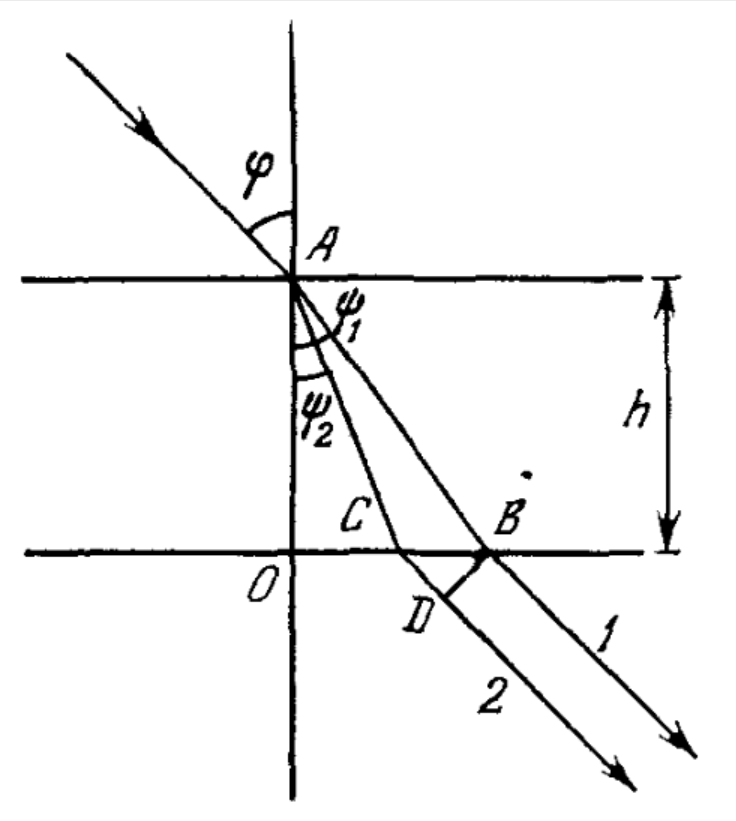
\includegraphics[width=1\textwidth]{images/intercolor.png}
    \caption{The crystal refract the beam differently.}
    %\label{fig:}
\end{figure}
\end{minipage}
\hfill
\begin{minipage}{0.55\textwidth}
    Going through the crystal plate the light gains the phase difference of
    \begin{equation*}
    	\Delta = h (n_2 \cos \psi_2 - n_1 \cos \psi_1),
    \end{equation*}
    for different refraction coefficient and refracting angles that have a small difference, so
    \begin{equation*}
    	\Delta = h \cos \psi (n_2 - n_1).
    \end{equation*}
\end{minipage}
